\documentclass[dvipsnames,table]{include/thesisclass} %compile with lualatex
\usepackage{media9}
%\usepackage[dvipsnames,table]{xcolor} %option clash with media9

\usepackage{listings}
\usepackage{float}
\usepackage{pdfpages}
\usepackage{subcaption}

%for tables
\usepackage{tabularx}
\usepackage{dcolumn,booktabs}
\renewcommand\thempfootnote{\arabic{mpfootnote}}
\newcolumntype{d}[1]{D{.}{.}{#1}}
\newcommand\mc[1]{\multicolumn{1}{c}{#1}} % handy shortcut macro

%misc
\usepackage{siunitx}
\sisetup{range-phrase=--} %used for \SIrange{1}{2}{\volt}
\DeclareSIUnit{\sample}{S}
\DeclareSIUnit{\bits}{B}
\usepackage{nicefrac}
\usepackage{amsmath}
\usepackage[normalem]{ulem}
\usepackage[figuresright]{rotating}
\usepackage{lscape}
\usepackage{textcomp}
\usepackage{trfsigns}
\usepackage{enumitem}
\newcommand{\thz}{\si{\tera\hertz}}
\newcommand{\eqdev}{\mathrel{\widehat{=}}}

%tikz & pgfplots
\usepackage{wrapfig}
\usepackage{tikz,tikzscale,pgfplots,pgfplotstable,tikz-timing}
\usepackage[european,siunitx]{circuitikz}
\usetikzlibrary{arrows,shapes,shadows,external,decorations.pathmorphing, positioning}
\tikzexternalize[optimize=false,prefix=tikz/]
\usetikztiminglibrary{arrows, clockarrows, nicetabs}
\pgfplotsset{compat=1.11}

\usetikzlibrary{fadings}
\tikzfading %strangely gives bad bounding box when inside the tikzpicture
[
name=fade out,
inner color=transparent!0,
outer color=transparent!100
]


\usepgfplotslibrary{units,fillbetween,colormaps} 
\pgfplotsset{compat=newest}

\pgfdeclarehorizontalshading{visiblelight}{50bp}{
	color(0.00000000000000bp)=(violet);
	color(8.33333333333333bp)=(blue);
	color(16.66666666666670bp)=(cyan);
	color(25.00000000000000bp)=(green);
	color(33.33333333333330bp)=(yellow);
	color(41.66666666666670bp)=(orange);
	color(50.00000000000000bp)=(red)
} 

\lstset{%
	breaklines=true,
	breakatwhitespace=true,
}

\renewcommand{\subsectionautorefname}{\sectionautorefname}
\renewcommand{\subsubsectionautorefname}{\sectionautorefname}




\SelectLanguage{english}
% details on this thesis
\newcommand{\thesisauthor}{Olena Manzhura}
\newcommand{\thesisentopic}{A Terabit Sampling System with a Photonics Time-Stretch ADC}
%\newcommand{\thesisentopic}{Ein Terabit Abtastsystem mit Photonic-Time-Stretch Analog-Digital-Wandler}
\newcommand{\thesislongtopic}{}
\newcommand{\thesisinstitute}{Institute for Data Processing and Electronics (IPE)}
\newcommand{\thesisreviewerone}{Prof. Dr. Anke-Susanne Müller (LAS)}
\newcommand{\thesisreviewertwo}{Dr. Michele Caselle (IPE)}
\newcommand{\thesisadvisorone}{} % to use: enter names and uncomment in titlepg
\newcommand{\thesisadvisortwo}{}
\newcommand{\thesistimestart}{15.11.2020} % on titlepage
\newcommand{\thesistimeend}{13.08.2021} % on titlepage
\newcommand{\thesistimehandin}{13.08.2021} % on second page 'preamble'
\newcommand{\thesispagehead}{Master Thesis: \thesisentopic} % page heading


\let\Oldsection\section
\renewcommand{\section}{\FloatBarrier\Oldsection}
\let\Oldsubsection\subsection
\renewcommand{\subsection}{\FloatBarrier\Oldsubsection}
\let\Oldsubsubsection\subsubsection
\renewcommand{\subsubsection}{\FloatBarrier\Oldsubsubsection}


\hypersetup
{
	pdfauthor={\thesisauthor},
	pdftitle={Masterarbeit: \thesisentopic},
	pdfsubject={\thesislongtopic},
	pdfkeywords={kit,etit,master,thesis,\thesisauthor}
}
\hyphenation
{
	über-nom-me-nen an-ge-ge-be-nen
}
\DeclareSIUnit{\sample}{S}
\sisetup{per-mode=symbol}

% acronyms
\usepackage[acronym,nomain,toc]{glossaries}
\glstoctrue






\setcounter{tocdepth}{2}



\begin{document}
\begin{tikzpicture}
	\node{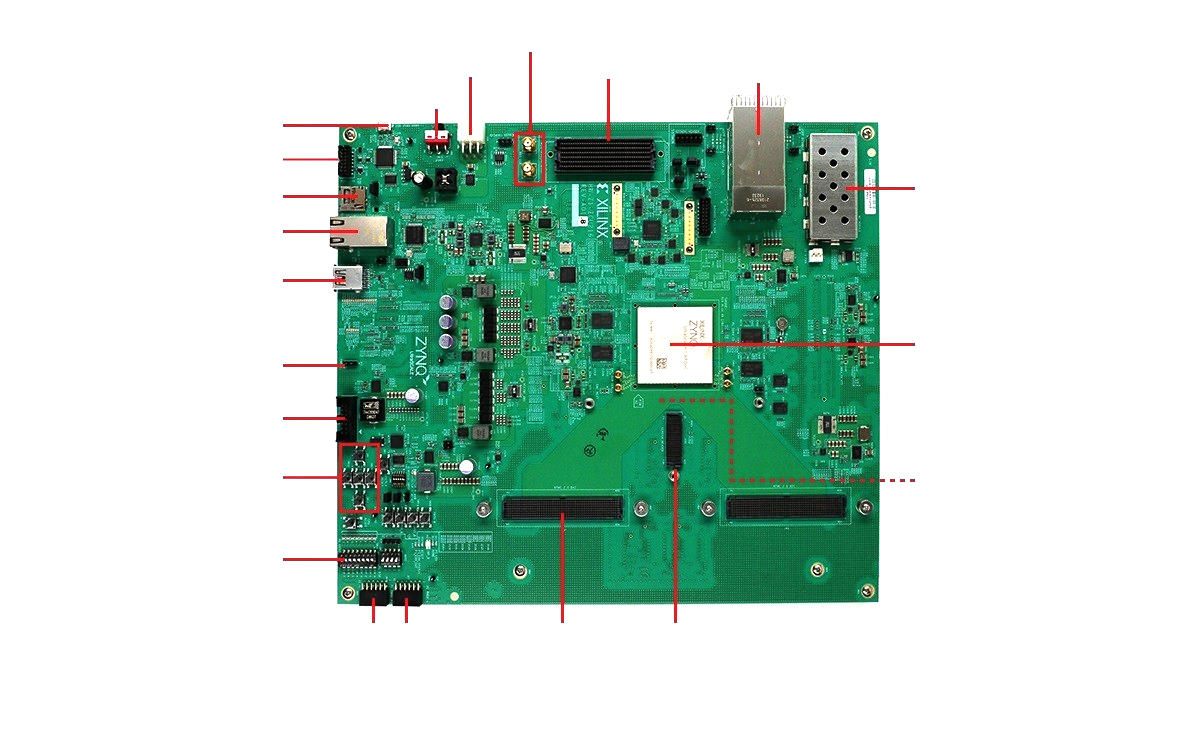
\includegraphics[width=8cm]{chap/05-readout/img/zcu216-cleared}};
	
	%left
	\node[fill=none,font=\tiny,align=right,anchor=east] at (-2.1,1.6) {USB (JTAG/UART)};
	\node[fill=none,font=\tiny,align=right,anchor=east] at (-2.1,1.38) {JTAG PC4};
	\node[fill=none,font=\tiny,align=right,anchor=east] at (-2.1,1.13) {Micro SD};
	\node[fill=none,font=\tiny,align=right,anchor=east] at (-2.1,0.9) {Ethernet};
	\node[fill=none,font=\tiny,align=right,anchor=east] at (-2.1,0.58) {USB 3.0};
	\node[fill=none,font=\tiny,align=right,anchor=east] at (-2.1,0) {PMBUS};
	\node[fill=none,font=\tiny,align=right,anchor=east] at (-2.1,-0.35) {MSP430 JTAG};
	\node[fill=none,font=\tiny,align=right,anchor=east] at (-2.1,-0.74) {Push Buttons};
	\node[fill=none,font=\tiny,align=right,anchor=east] at (-2.1,-1.28) {User 8-pole\\DIP Switch};
	
	%bottom
	\node[fill=none,font=\tiny,align=center,anchor=north] at (-1.39,-1.7) {Pmods ($2 \times$)};
	\node[fill=none,font=\tiny,align=center,anchor=north] at (-0.24,-1.7) {RFMC 2.0\\(DAC)};
	\node[fill=none,font=\tiny,align=center,anchor=north] at (0.51,-1.7) {CLK104 \\ Connector};
	\node[fill=none,font=\tiny,align=center,anchor=north] at (1.26,-1.7) {RFMC 2.0\\(ADC)};
	
	%right
	\node[fill=none,font=\tiny,align=left,anchor=west] at (2.13,1.19) {SATA M.2};
	\node[fill=none,font=\tiny,align=left,anchor=west] at (2.13,0.14) {XCZU49DR-2FFVF1760E};
	\node[fill=none,font=\tiny,align=left,anchor=north west] at (2.13,-0.6) {Under the board:\\DDR4 4$\times$ 8-bit Clamshell\\Component Memory (4 GB)\\[2ex]DDR4 4$\times$ 8-bit Clamshell\\Component Memory (4 GB)\\[2ex]DDR4 SODIMM Socket with\\64-bit DDR4 SODIMM};
	
	%top
	\node[fill=none,font=\tiny,align=center,anchor=south] at (1.07,1.91) {SFP28 (4$\times$)};
	\node[fill=none,font=\tiny,align=center,anchor=south] at (0.07,1.91) {FMC+};
	\node[fill=none,font=\tiny,align=center,anchor=south] at (-0.45,2.13) {SMA\\MGMT\\CLK};
	\node[fill=none,font=\tiny,align=center,anchor=south] at (-0.85,1.91) {12 V};
	\node[fill=none,font=\tiny,align=center,anchor=south east] at (-0.98,1.64) {Power\\Switch};
\end{tikzpicture}
\end{document}
